\documentclass{article}

\usepackage{arxiv}

\usepackage[spanish]{babel}
\usepackage[utf8]{inputenc} % allow utf-8 input
\usepackage[T1]{fontenc}    % use 8-bit T1 fonts
\usepackage{hyperref}       % hyperlinks
\usepackage{url}            % simple URL typesetting
\usepackage{booktabs}       % professional-quality tables
\usepackage{amsfonts}       % blackboard math symbols
\usepackage{nicefrac}       % compact symbols for 1/2, etc.
\usepackage{microtype}      % microtypography
\usepackage{lipsum}
\usepackage{graphicx}
\graphicspath{ {./images/} }


\title{TP 1.1 - SIMULACIÓN DE UNA RULETA}


\author{
    Alvaro Tomasino \\
    Ingeniería en Sistemas de Información\\
    Universidad Tecnológica Nacional - FRRO\\
    Zeballos 1341, S2000, Argentina\\
    \texttt{atomasino08@gmail.com} \\
\And
    Melina Aronson \\
    Ingeniería en Sistemas de Información\\
    Universidad Tecnológica Nacional - FRRO\\
    Zeballos 1341, S2000, Argentina\\
    \texttt{melinaaronson@gmail.com} \\
\And
    Tomas Aguilera \\
    Ingeniería en Sistemas de Información\\
    Universidad Tecnológica Nacional - FRRO\\
    Zeballos 1341, S2000, Argentina\\
    \texttt{tomas.aguilera.27@gmail.com} \\
\And
    Juan Bautista Martinelli \\
    Ingeniería en Sistemas de Información\\
    Universidad Tecnológica Nacional - FRRO\\
    Zeballos 1341, S2000, Argentina\\
    \texttt{yul217@pitt.edu} \\
}




\begin{document}

\maketitle




\begin{abstract}
  El siguiente documento tiene como objetivo detallar el trabajo de investigación realizado como introducción a la 
  materia de simulación. El mismo consiste en el desarrollo de un modelo simple del plato de una ruleta, cuyo 
  funcionamiento es verificado mediante distintos tests rudimentarios.
\end{abstract}

\keywords{Simulación \and Trabajo de investigación \and Ruleta}






\section{Introducción}
\paragraph{Etimología y definición del término ruleta} La ruleta \cite{ruleta_wiki} es un juego de azar típico de 
los casinos, cuyo nombre viene del término francés \textit{roulette}, que significa «ruedita» o «rueda pequeña». 
Su uso como elemento de juego de azar, aún en configuraciones distintas de la actual, no está documentado hasta 
bien entrada la Edad Media. Es de suponer que su referencia más antigua es la llamada Rueda de la Fortuna, de la que 
hay noticias a lo largo de toda la historia, prácticamente en todos los campos del saber humano.

\paragraph{Popularización y asociaciones}
La «magia» del movimiento de las ruedas debió impactar a distintas generaciones. La aparente quietud del centro, el 
aumento de velocidad a medida que nos alejamos de él y la posibilidad de que se detenga en un punto al azar tuvieron 
que influir en el desarrollo de diversos juegos basados en la rueda.

Las ruedas, y por extensión las ruletas, siempre han estado vinculadas con el mundo mágico y esotérico. Así, una de 
ellas forma parte del tarot, más precisamente de los denominados arcanos mayores.

\paragraph{Evolución de las reglas de juego a través de la historia} Según los indicios, la creación de una ruleta y 
sus normas de juego, muy similares a las que conocemos hoy en día, se debe a Blaise Pascal, matemático francés, quien 
ideó una ruleta con treinta y seis números (sin el cero), en la que hay un extremo equilibrio en la posición en que está 
colocado cada número. La elección de 36 números da un alcance aún más vinculado a la magia (la suma de los primeros 36 
números da el número mágico por excelencia: seiscientos sesenta y seis).

Esta ruleta podía usarse como entretenimiento en círculos de amistades. Sin embargo, a nivel de empresa que pone los 
medios y el personal para el entretenimiento de sus clientes, no era rentable, ya que estadísticamente todo lo que se 
apostaba se repartía en premios (probabilidad de 1/36 de acertar el número y ganar 36 veces lo apostado).

En 1842, los hermanos Blanc modificaron la ruleta añadiéndole un nuevo número, el 0, y la introdujeron inicialmente 
en el Casino de Montecarlo. Esta es la ruleta que se conoce hoy en día, con una probabilidad de acertar de 1/37 y ganar
36 veces lo apostado, consiguiendo un margen para la casa del 2,7\% (1/37).

Más adelante, en algunas ruletas (sobre todo las que se usan en países anglosajones) se añadió un nuevo número 
(el doble cero), con lo cual el beneficio para el casino resultó ser doble (2/38 o 5,26\%).

\paragraph{Tipos de juegos de ruleta} En la actualidad, existen dos tipos de ruletas: La \textit{ruleta francesa}, también 
llamada \textit{ruleta europea}, y la \textit{ruleta americana}.

La ruleta europea está compuesta por 37 números: del 1 al 36 y el cero. En cambio, la ruleta americana tiene dos variantes: 
la ruleta americana de \textit{doble cero} (compuesta por 38 números: los números del 1 al 36, el cero y el doble cero) y la 
de \textit{un cero} (compuesta por 37 números: del 1 al 36 y el cero, al igual que la europea).

\begin{figure}[h]
  \centering
  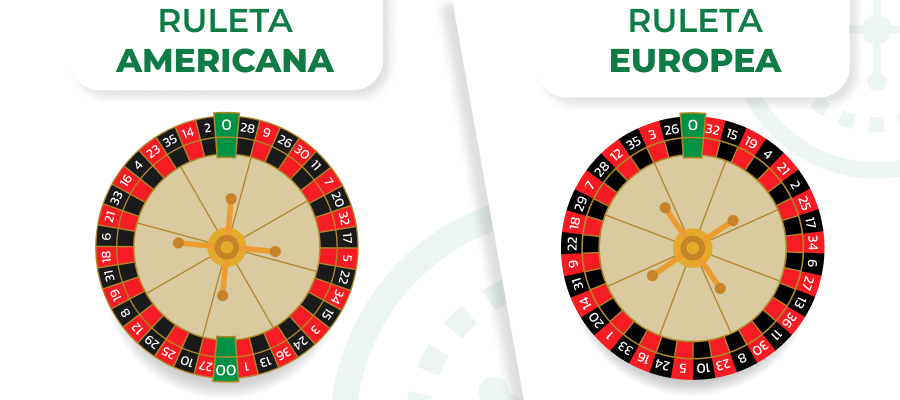
\includegraphics[width=0.8\textwidth]{ruleta-americana-vs-europea.jpg}
  \caption{Diferencias entre la ruleta americana y la ruleta europea \cite{tipos_de_ruleta_casino}.}
  \label{fig:tipos-de-ruleta}
\end{figure}

En Argentina se juega principalmente la ruleta europea, que es la más común en los casinos del país.
Debido a ello, este informe se realizó basado en la ruleta europea; por lo tanto, en adelante, cuando
hablemos de ruleta, nos estaremos refiriendo a este tipo.

La simulación analizada no es simplemente un programa de generación de números al 
azar: es una implementación computacional de los principios fundamentales de la estadística descriptiva e inferencial. Cada 
variable del código tiene un correlato teórico preciso en la teoría de la probabilidad.

La distribución uniforme discreta sobre $\{0,1,2,\dots,36\}$ determina todos los valores teóricos del sistema. 
Las frecuencias absoluta y relativa son las herramientas empíricas para aproximar la probabilidad desde los datos. 
El valor promedio, la varianza y el desvío estándar permiten caracterizar globalmente el comportamiento de la variable. 
Finalmente, el Teorema Central del Límite es el principio que garantiza la coherencia entre la teoría y el experimento simulado.

Comprender estos conceptos es esencial tanto para interpretar correctamente los resultados de cualquier simulación como para 
diseñar experimentos computacionales que sean estadísticamente significativos.


\section{Métodos}
\label{sec:headings}

\subsection{Diseño del modelo}
El modelo fue construido en el lenguaje \textit{Python 3.x}, siguiendo los requisitos de generación de 
valores aleatorios enteros y el uso de listas para el almacenamiento de datos.

Utilizamos las siguientes librerías: \textit{argparse}, \textit{numpy} y \textit{matplotlib}.

Estas librerías forman un conjunto de herramientas esenciales para el desarrollo de aplicaciones en \textit{Python}, 
permitiendo desde la interacción con el entorno hasta el análisis avanzado de datos. \textit{argparse} facilita la 
creación de interfaces de línea de comandos profesionales para capturar argumentos del usuario.
\textit{numpy} introduce estructuras de datos de alto rendimiento, como los \textit{arrays} multidimensionales, que 
permiten realizar operaciones matemáticas complejas de manera mucho más eficiente que las listas estándar de \textit{Python}. 
Para dar sentido a estos datos, \textit{matplotlib.pyplot} se utiliza para generar gráficos, diagramas de dispersión, 
histogramas o series temporales, permitiendo una interpretación visual de la información procesada.
Para la ejecución del programa se deberá ejecutar el siguiente comando: 
\begin{center}
  \textit{python ruleta.py -c XXX -n YYY -e ZZ}
\end{center}
\begin{itemize}
  \item Número de tiradas o número de la muestra (\textit{n}): XXX.
  \item Cantidad de corridas o \textit{realization} (\textit{c}): YYY.
  \item Número elegido o apuesta (\textit{e}): ZZZ.
\end{itemize}

El programa permite la interacción mediante la consola de comandos, recibiendo 3 parámetros:
\textit{XXX} la cantidad de tiradas de la ruleta o número de la muestra (\textit{n}), \textit{YYY} la cantidad de corridas 
o \textit{realization} de la simulación (\textit{c}) y \textit{ZZ} el número elegido en la ruleta ($e\in\{0,1,2,\dots,36\}$), al que vamos a apostar 
nuestro dinero.


\subsubsection{Procesamiento de datos}

\paragraph{Paragraph}

\section{Resultados}
\label{sec:others}

The documentation for \verb+natbib+ may be found at
\begin{center}
  \url{http://mirrors.ctan.org/macros/latex/contrib/natbib/natnotes.pdf}
\end{center}
Of note is the command \verb+\citet+, which produces citations
appropriate for use in inline text.  For example,
\begin{verbatim}
   \citet{hasselmo} investigated\dots
\end{verbatim}
produces
\begin{quote}
  Hasselmo, et al.\ (1995) investigated\dots
\end{quote}

\begin{center}
  \url{https://www.ctan.org/pkg/booktabs}
\end{center}


\subsection{Figures}
\lipsum[10]
See Figure \ref{fig:fig1}. Here is how you add footnotes. \footnote{Sample of the first footnote.}
\lipsum[11]

%\begin{figure} % picture
%    \centering
%    \includegraphics{test.png}
%\end{figure}

\subsection{Lists}
\begin{itemize}
  \item Lorem ipsum dolor sit amet
  \item consectetur adipiscing elit.
  \item Aliquam dignissim blandit est, in dictum tortor gravida eget. In ac rutrum magna.
\end{itemize}

\subsection{Tables}
\lipsum[12]
See awesome Table.
\begin{table}
  \caption{Sample table title}
  \centering
  \begin{tabular}{lll}
    \toprule
    \multicolumn{2}{c}{Part}                   \\
    \cmidrule(r){1-2}
    Name     & Description     & Size ($\mu$m) \\
    \midrule
    Dendrite & Input terminal  & $\sim$100     \\
    Axon     & Output terminal & $\sim$10      \\
    Soma     & Cell body       & up to $10^6$  \\
    \bottomrule
  \end{tabular}
  \label{tab:table}
\end{table}

\section{Discusión}

\section{Conclusiones}

\nocite{*}

\bibliographystyle{unsrt}
\bibliography{references}

\end{document}


